\section{Inverse Design for Elastostatics}
Given a set of base materials, an object layout, and functional objectives, the goal of inverse design is to compute the material distribution inside the object that optimizes the objectives.
In our approach, instead of computing per-voxel base material distribution, we work with microstructures made of the base materials and the space of physical material properties spanned by them. The complete pipeline of our system, illustrated in Figure \ref{fig:topoptOverview}, can be decomposed into two stages---gamut generation and gamut-constrained topology optimization.
\begin{figure}[hb]
	\centering
	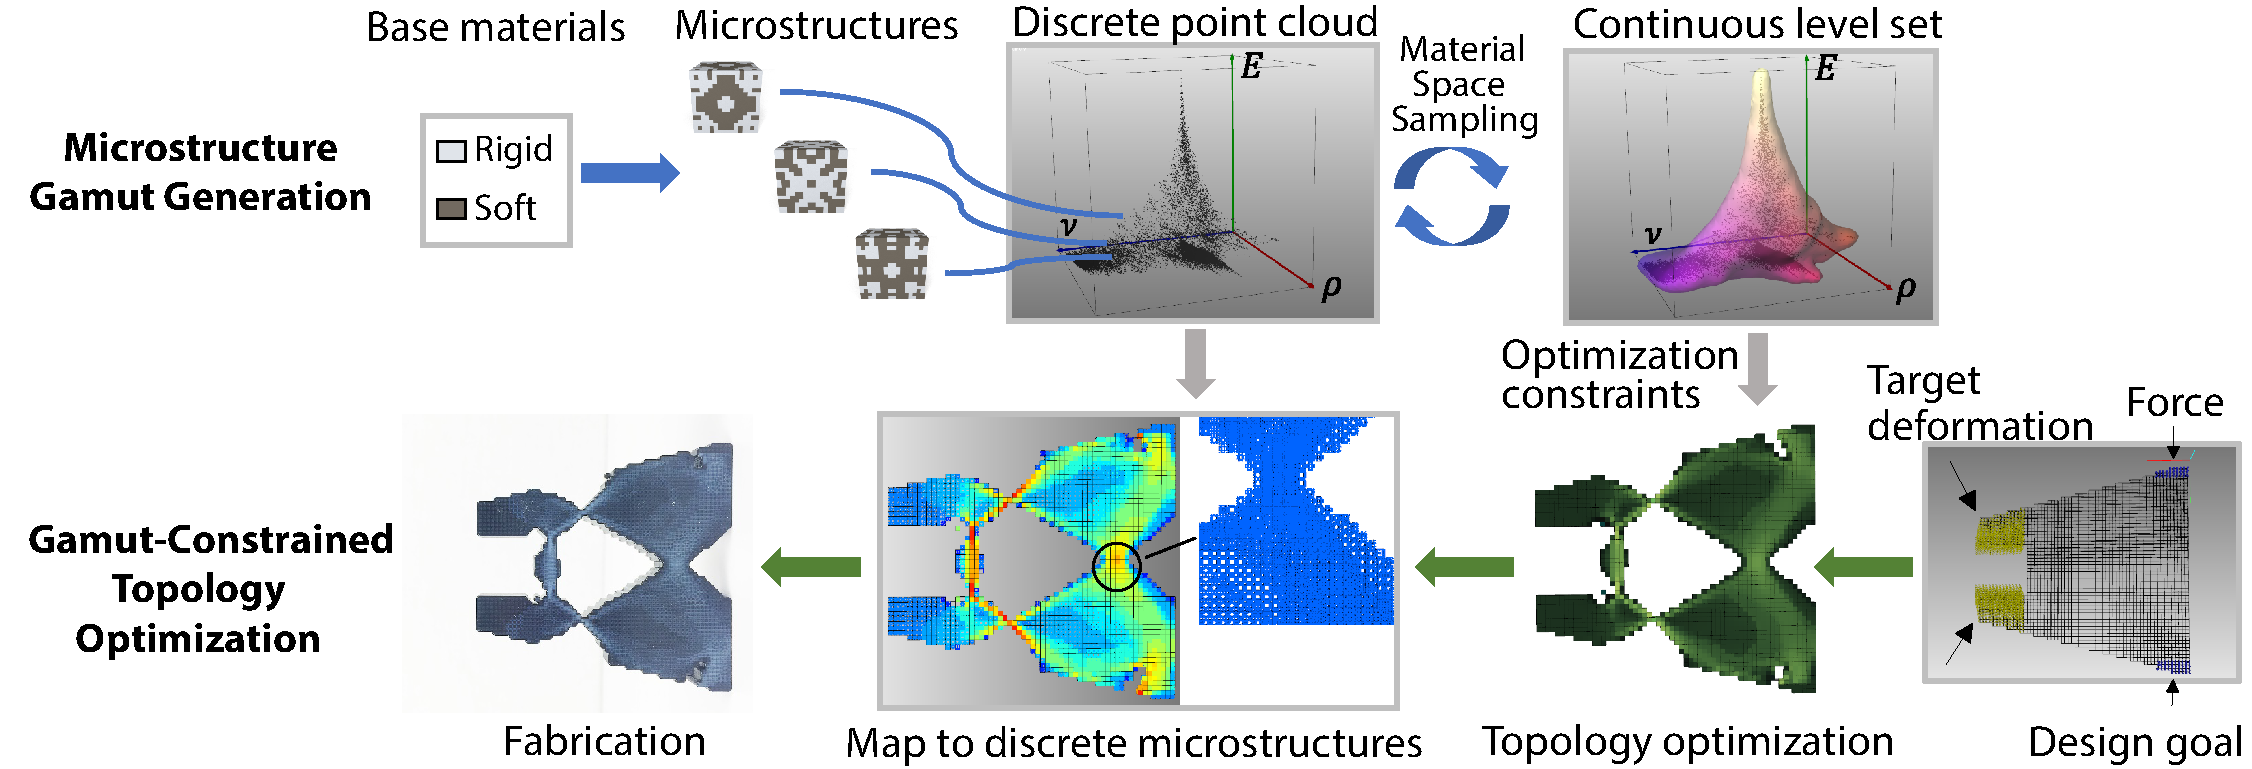
\includegraphics[width=0.95\textwidth]{images/topoptOverview.pdf}
	\caption{Inverse design algorithm.}
	\label{fig:topoptOverview}
\end{figure}
\subsection{Gamut Exploration}
In the first stage, we estimate the gamut of material properties covered by all possible microstructures made by spatial arrangement of base materials. 
Since exhaustively computing the properties of all these microstructures is, in practice, intractable, we progressively increase the material space by alternating a stochastic search and a continuous optimization. The first step introduces discrete changes in the materials of the microstructures and allows emergence of new types of microstructures. The second step allows to locally push the material space boundaries by refining the microstructure shapes. After completing this stage, we obtain a discrete representation of the space of material properties and the mapping between these properties and the corresponding microstructures.

\subsection{Gamut-Constrained Topology Optimization}
In the second stage, we construct a smooth continuous gamut representation of the material property space by using a level set field. We define our topology optimization problem directly in this space. Our approach minimizes the objective function over possible material parameters while asking for strict satisfaction of the physics constraints -- typically, the static equilibrium -- as well as the strict satisfaction of the physical parameter bounds. Taking advantage of our gamut representation as a level set, we formulate this last constraint as limiting the material properties to stay on the negative side of the level set. This guarantees that the material properties that we use in the optimization are always physically realizable.


\subsection{Discovering Families of Extremal Structures}
\begin{figure}[ht]
	\centering
	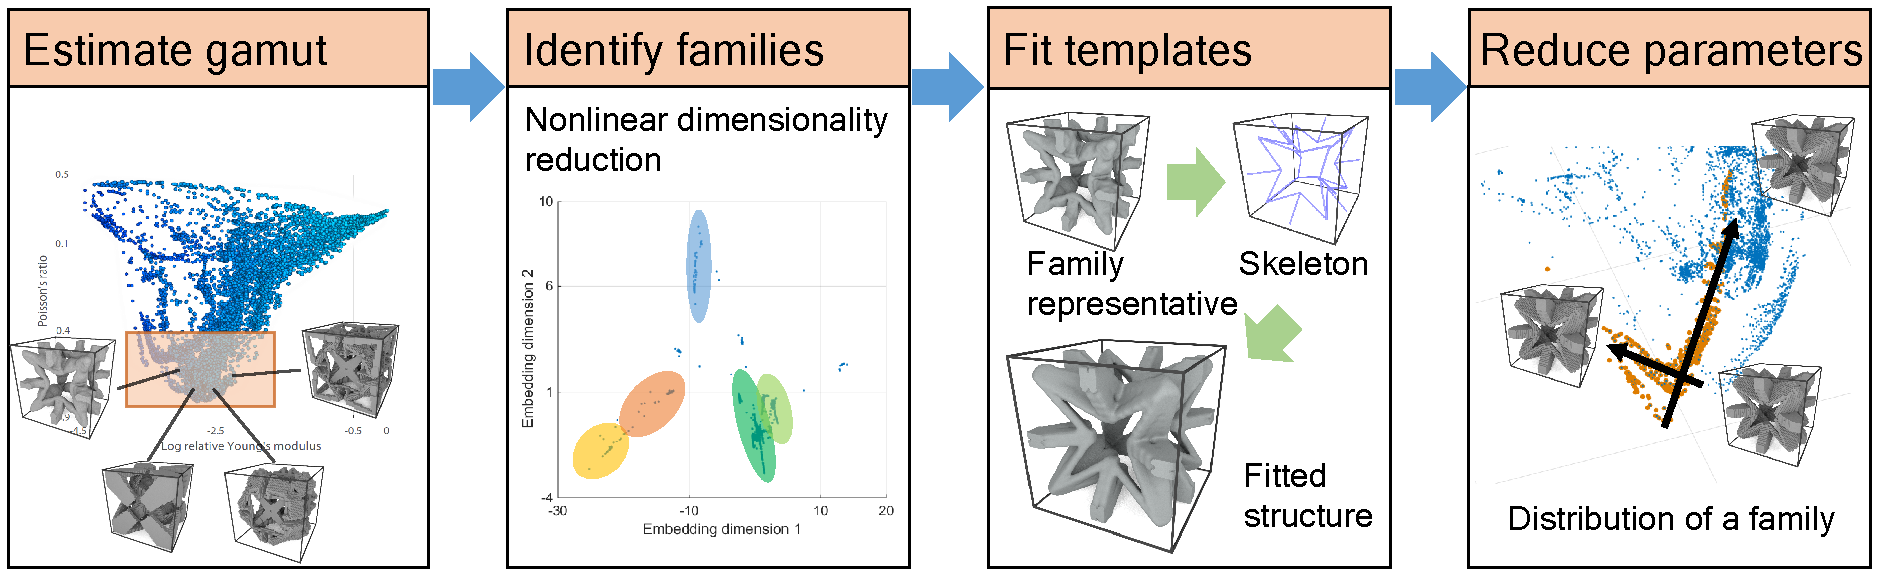
\includegraphics[width=0.9\textwidth]{images/discoverPipe.pdf}
	\caption{A computational process for discovery of extremal microstructure families. Given a set of physical properties and design constraints, we estimate the material property gamut using stochastic sampling and topology optimization. Structures near the gamut boundary are grouped into families using nonlinear dimensionality reduction. A representative from each family is fitted with a template represented as a skeleton. Beams are placed on the skeleton edges with optimized parameters to fit the original structure. Structure variations with the same topology can be generated by varying the beam parameters. Finally, reduced template parameters are computed to reveal domain-specific design principles}
	\label{fig:discoverFamily}
\end{figure}
In addition to facilitating gamut-constrained topology optimization, 
the microstructure gamut enables discovery of 
families of structures with extremal physical properties.
Our discovery pipeline has four steps (Figure~\ref{fig:discoverFamily}).
The first step estimates the material property gamut, which is the range of material properties achieved by microstructures. Here a microstructure is defined on a 3D regular grid composed of hexahedral voxels. The design space includes all possible material assignments to the voxels. Since exhaustively simulating all possible microstructures is impractical, this step computes a set of sample microstructures. The sampling algorithm alternates between topology optimization and stochastic discrete search to progressively expand the gamut~\cite{Zhu2017}. The topology optimization stage pushes structures towards outside of the gamut boundary along gradient directions. The stochastic stage introduces discrete changes to escape local optima.

In the second step, common geometric traits are identified among microstructures near the gamut boundary. Geometrically similar structures are grouped into families using nonlinear dimensionality reduction (NLDR). Isomap~\cite{tenenbaum2000global} is used as the reduction method because it can discover long sequences of related structures while keeping distant points separated. The effectiveness of NLDR depends on the distance metric that measures geometric difference. A smoothed Euclidean norm is chosen for robustness (figure S1). NLDR outputs an embedding of the microstructures in a low-dimensional space where similar structures are closely packed. Microstructures in the embedding space are clustered using a Gaussian mixture model~\cite{mclachlan2007algorithm} where each cluster corresponds to a family. Families with a significant number ($\geq 200$) of members are extracted for further analysis.

The third step in our process constructs templates for each microstructure family. We observe that most of the extremal structures are composed from beams, plates and blocks. All of these structures can be represented as cuboids with different edge lengths. We therefore chose cuboids as the building blocks for microstructure templates, and note that some structures near the boundary do not fit the cuboid representation (figure. S4).
To find a template from a family representative, its topology is computed using a morphological skeleton~\cite{Lee1994Skel}.
The morphological skeleton is a set of connected edges that largely preserves topological and branching characteristics of the structures. The skeleton is converted into a graph in order to represent a template. A cuboid is placed on each edge of the graph with optimized sizing and orientation to best match the representative structure. More details of the process are available in the supplementary text.

Finally, reduced parameters are computed to allow an intuitive navigation in the material property space. Since the templates from the previous step contain tens of parameters that do not directly correspond to material properties, it is still difficult to understand the key design principles. The reduced parameters allow for direct tuning of each material property. For a given parametric template, its parameters are fitted to all structures of the corresponding family. Principal component regression (PCR) is then performed on the set of fitted template parameters to find principal directions in the template parameters space. Varying the parameters in a direction corresponds to moving on the gamut boundary in a certain direction. A reduced parameter is assigned to each direction to control amount of change along that direction.